\documentclass[10pt,a4paper]{article}
\usepackage[natbibapa]{apacite} 
\usepackage{amsmath}
\usepackage{textcomp}
\usepackage[a4paper,margin=0.8in]{geometry} 
\usepackage{latexsym}
\usepackage{tikz}
\usepackage{etoolbox}

%opening
\title{COS 4807 Assignment 2}
\author{Adriaan Louw (53031377)}

\newcommand{\interp}{I}


\tikzset{
  treenode/.style = {shape=rectangle, rounded corners,
                     draw, align=center,
                     top color=white, bottom color=blue!20},
  root/.style     = {treenode, font=\Large, bottom color=red!30},
  env/.style      = {treenode, font=\ttfamily\normalsize},
  dummy/.style    = {circle,draw}
}

\usetikzlibrary{shapes.misc}


\begin{document}

\maketitle


\section{Question 1}

\begin{equation}
 ((p\wedge q)\rightarrow r) \rightarrow (p \rightarrow (q\vee r))
\end{equation}

\begin{equation}
 \neg((p \wedge q) \rightarrow r) \vee (p\rightarrow(q\vee r))
\end{equation}

\begin{equation}
 \neg (\neg(p \wedge q) \vee r) \vee (\neg p \vee (q\vee r))
\end{equation}

\begin{equation}
 ((p\wedge q) \wedge(\neg r))\vee (\neg p \vee q \vee r)
\end{equation}

\begin{equation}
 ((\neg p \vee q \vee r)\vee (p \wedge q))\wedge ((\neg p \vee q \vee r) \vee \neg r)
\end{equation}

\begin{equation}
 ((\neg p \vee q \vee r)\vee (p \wedge q))\wedge (true)
\end{equation}

\begin{equation}
 ((\neg [ \vee q \vee r)\vee p)\wedge((\neg p \vee q \vee r )\vee q)
\end{equation}

\begin{equation}
 (true)\wedge((\neg p \vee q \vee r )\vee q)
\end{equation}

\begin{equation}
((\neg p \vee q \vee r )\vee q)
\end{equation}

\begin{equation}
\{\{\neg p, q,r\}\}
\end{equation}

Which in abreviated clausal form is $\{\bar{p}qr\}$.

\section{Question 2}

\begin{equation}
 \neg ((q\rightarrow p)\rightarrow r)\wedge ((p \wedge \neg r)\rightarrow (q\wedge r))
\end{equation}

\begin{equation}
 \neg(\neg(p\rightarrow p) \vee r) \wedge (\neg(p\wedge \neg r) \vee (q\wedge r))
\end{equation}

\begin{equation}
\neg(\neg(\neg q \vee p)\vee r)\wedge ((\neg p \vee r)\vee (q\wedge r))
\end{equation}

\begin{equation}
 (\neg q\vee p) \wedge (\neg r) \wedge (((\neg p \vee r)\vee q)\wedge((\neg p \vee r)\vee r))
\end{equation}

\begin{equation}
 (\neg q\vee p) \wedge (\neg r) \wedge (\neg p\vee q\vee r) \wedge(\neg p\vee r)
\end{equation}

Which is $\{\{p,\neg q\},\{\neg r\},\{\neg p,q,r \},\{\neg p,r\}\}$ in clausal form


\begin{tabular}{ll}
1. $p\bar{q}$  &\\
2. $\bar{r}$   &\\
3. $\bar{p}qr$ &\\
4. $\bar{p}r$  &\\
5. $\bar{p}$   &           2 and 4\\
6. $\bar{q}$   &           1 and 5\\
7. $\bar{p}r$  &           3 and 6\\
8. $\bar{p}$   &           2 and 7\\
9. $\bar{q}r$  &           1 and 4\\
10 $\bar{q}$   &           2 and 9\\
\end{tabular}

No boxes have been found so this formula must be satisfiable

\section{Question 3}

Forumla A:

\begin{equation}
 p\rightarrow q
\end{equation}

\begin{equation}
 \neg p\vee q
\end{equation}

$\{\bar{p}q\}$

Formula B:

\begin{equation}
 q \rightarrow r
\end{equation}

\begin{equation}
 \neg q \vee r
\end{equation}


$\{\bar{q}r\}$


Negation of the single formula

\begin{equation}
 \neg(p\rightarrow (q\wedge r))
\end{equation}

\begin{equation}
 \neg(\neg p \vee (q \wedge r))
\end{equation}

\begin{equation}
 p \wedge (\neg q\vee r)
\end{equation}

\begin{equation}
 (p\wedge \neg q)\vee (p\wedge \neg r)
\end{equation}

\begin{equation}
 ((p\wedge \neg q) \vee p)\wedge((p\wedge\neg q)\vee \neg r)
\end{equation}

\begin{equation}
 (p\vee p)\wedge (p\vee \neg q)\wedge(\neg r \vee p)\wedge (\neg r \vee \neg q)
\end{equation}

Which is $\{p,p\bar{q},p\bar{r},\bar{q}\bar{r} \}$

Now for the resolution refutation


\begin{tabular}{ll}
1. $p$  &\\
2. $p\bar{q}$   &\\
3. $p\bar{r}$ &\\
4. $\bar{q}\bar{r}$  &\\
5. $\bar{p}q$   &           \\
6. $\bar{q}r$   &           \\
7. $q$  &           1 and 5\\
8. $q\bar{r}$   &           3 and 5\\
9. $\bar{r}$  &           4 and 7\\
10 $\bar{r}$   &           4 and 8\\
11 $r$   &           6 and 7\\
12 $\Box$   &           10 and 11\\
\end{tabular}

Because resolution refutation shows that the set of clauses is unsatidfiable we can conslude that 
$\{p\rightarrow q,q \rightarrow r\} \models p \rightarrow (q \wedge r)$

\section{Question 4}

For 

\begin{equation}
(p\vee q)\rightarrow r 
\end{equation}

using ordering (p,q,r)



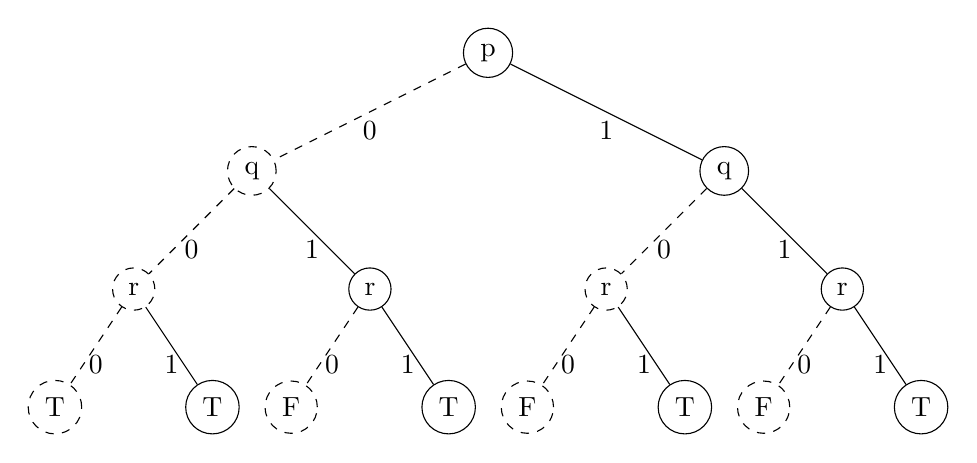
\begin{tikzpicture}
 [level/.style={sibling distance=60mm/#1}]
 
 \node [circle,draw] {p}
    child[dashed] { node [circle,draw] {q}
      child[dashed] { node[dummy] {r}
      	 child[dashed] { node[dummy] {T}
         	edge from parent node [below] {0} }
         child[solid] { node[dummy] {T}
         	edge from parent node [below] {1} }
         edge from parent node [below] {0} }
      child[solid] { node[dummy] {r}
         child[dashed] { node[dummy] {F}
         	edge from parent node [below] {0} }
         child { node[dummy] {T}
         	edge from parent node [below] {1} }
         edge from parent node [below] {1} }    
      edge from parent node[below] {0} }
    child { node [circle,draw] {q}
      child[dashed] { node [dummy] {r}
         child[dashed] { node[dummy] {F}
         	edge from parent node [below] {0} }
         child[solid] { node[dummy] {T}
         	edge from parent node [below] {1} }
         edge from parent node [below] {0} } 
      child { node [dummy] {r}
         child[dashed] { node[dummy] {F}
         	edge from parent node [below] {0} }
         child { node[dummy] {T}
         	edge from parent node [below] {1} }
         edge from parent node [below] {1} }  
      edge from parent node[below] {1}};
\end{tikzpicture}





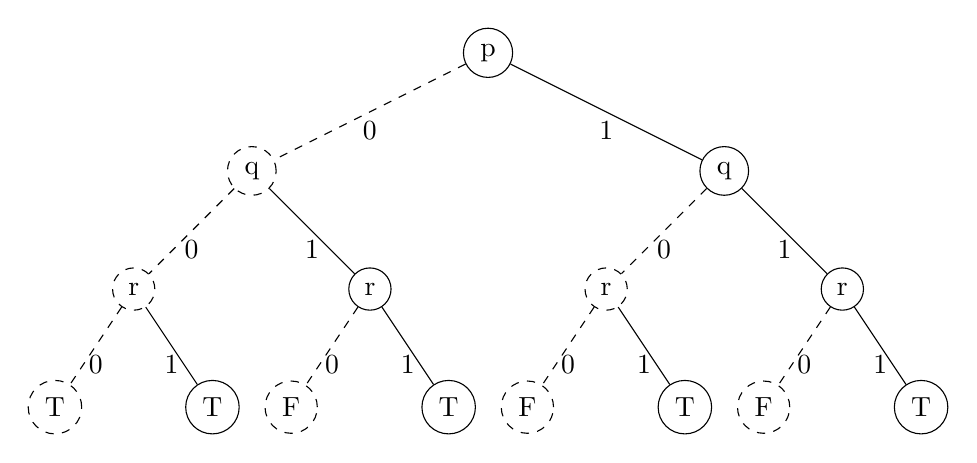
\begin{tikzpicture}
 [level/.style={sibling distance=60mm/#1}]
 
  \node [circle,draw] {p}
    child[dashed] { node [circle,draw] {q}
      child[dashed] { node[dummy] {r}
      	 child[dashed] { node[dummy] {T}
         	edge from parent node [below] {0} }
         child[solid] { node[dummy] {T}
         	edge from parent node [below] {1} }
         edge from parent node [below] {0} }
      child[solid] { node[dummy] {r}
         child[dashed] { node[dummy] {F}
         	edge from parent node [below] {0} }
         child { node[dummy] {T}
         	edge from parent node [below] {1} }
         edge from parent node [below] {1} }    
      edge from parent node[below] {0} }
    child { node [circle,draw] {q}
      child[dashed] { node [dummy] {r}
         child[dashed] { node[dummy] {F}
         	edge from parent node [below] {0} }
         child[solid] { node[dummy] {T}
         	edge from parent node [below] {1} }
         edge from parent node [below] {0} } 
      child { node [dummy] {r}
         child[dashed] { node[dummy] {F}
         	edge from parent node [below] {0} }
         child { node[dummy] {T}
         	edge from parent node [below] {1} }
         edge from parent node [below] {1} }  
      edge from parent node[below] {1}};
\end{tikzpicture}












\end{document}
